\subsection{Scoring in Detail}

The heuristic score is additive and every component is inspectable. A candidate starts at 0.8 for carrying at least one mechanism (+0.2 for a second, +0.2 for a third); +0.6 for deontic or decision language (\emph{should, must, need to, recommend, object, reject, accept, agree, insist, strongly, clearly}); +0.4 for justification language (\emph{because, therefore, for example, evidence, in practice, in my experience, shows that}); +0.5 for an explicit reference to the proposal (\emph{PEP~572, this change, this syntax, the spec}); +0.4 for a non-neutral direction; +0.2 for an internal or external scope and +0.4 for a mixed one; +0.3 for a recognised target; a role weight of 1.0 for the BDFL or Steering Council, 0.9 for a delegate, 0.8 for a core developer or release manager, 0.7 for a proposal author or PEP editor, 0.2 for a community member; +0.8, +0.5 or +0.2 when the message precedes a known decision by at most 7, 30 or 90 days; $-$0.2 for hedging (\emph{maybe, perhaps, not sure, I wonder}) and $-$0.3 for sentences shorter than six words unless they are votes. Unknown decision dates and post-decision messages add nothing, so proposals without a resolved decision are not boosted. The threshold of 1.0 keeps every sentence with a mechanism and at least one further signal; the annotation study will tell whether it should be raised.

\subsection{Tool Interfaces}

Influence Miner is delivered as a tab in both incarnations of the DeMaP Miner viewer, so that a candidate sentence is never more than one click away from the message it came from. In the Java desktop tool (Figure~\ref{fig:desktop}) the tab sits on the right-hand tabbed pane next to the existing \emph{Reasons}, \emph{InfluenceOfRoles} and \emph{SentimentOfMembers} tabs. Its controls filter by mechanism (including a \emph{Controversial (any of the 7)} option for the mechanisms of Section~\ref{sec:controversial}), direction, author role, governance era, minimum score and sort order; \emph{Load Influence Candidates} fills the results table of the viewer with the proposal's candidates (date, message id, author with role, mechanisms, direction, scope and target, sentence with its evidence cues, score) and a summary line gives the counts by mechanism and direction; \emph{Run Influence Miner for PEP} re-extracts the proposal in the background. Selecting a row loads the source message into the central viewer, exactly as for reason candidates, so that an analyst can read the sentence in its thread. In the web version (Figure~\ref{fig:web}), a Flask port of the same layout, the right-hand panel carries \emph{Reasons}, \emph{Preference Miner} and \emph{Influence Miner} tabs; the Influence Miner tab adds bar summaries of mechanisms and directions (controversial mechanisms highlighted in red), role and phase tags, a top-participants table and the candidate table with message links, and a separate overview page reports the corpus-wide distributions and the governance-era comparison of Section~\ref{sec:results}.3. Both interfaces read the same \texttt{influence\_candidates} table and can be pointed at either the original or the extended database.

\begin{figure*}[t]
\centering
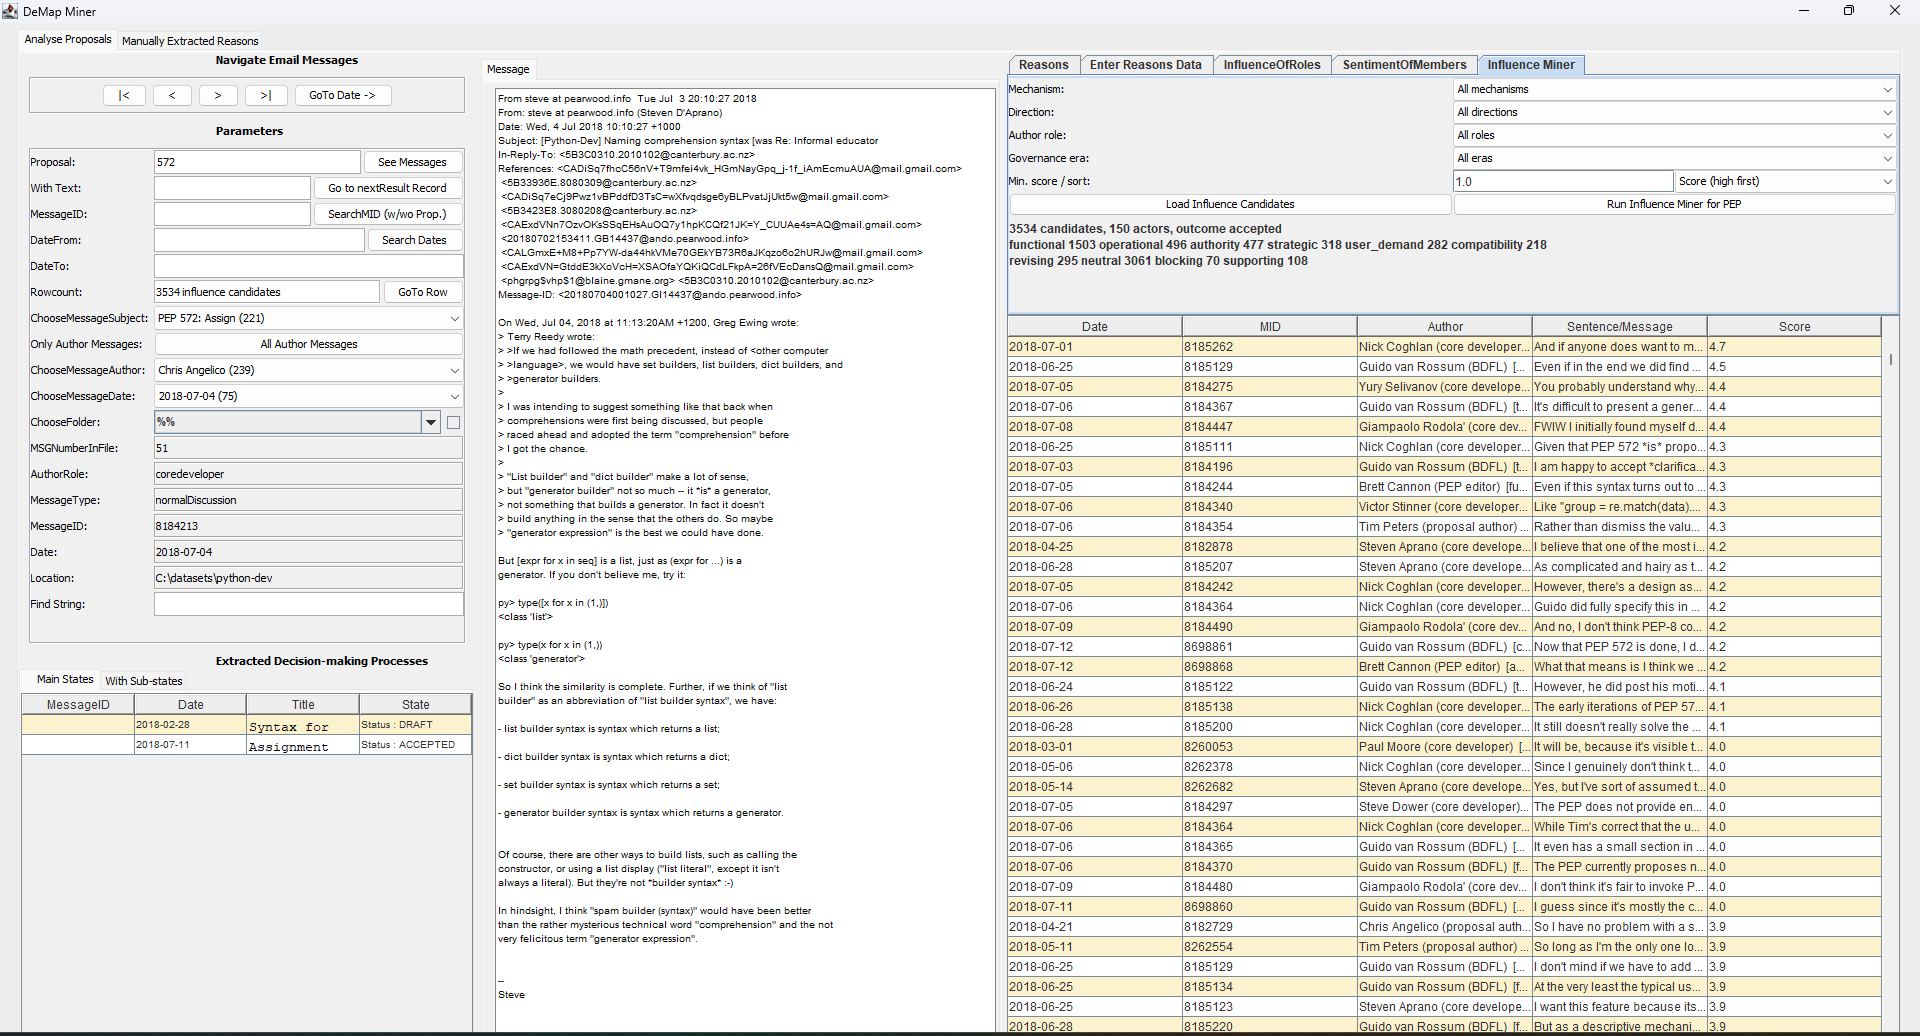
\includegraphics[width=\textwidth]{figures/fig_desktop_influence_tab_crop.png}
\caption{Influence Miner tab in the DeMaP Miner desktop tool (PEP~572, extended corpus). Right: filters, summary and the candidate table; centre: the message selected from the table; left: navigation, parameters and the PEP's state history.}
\Description{Screenshot of a Java Swing application with a maximised window: a left navigation panel, a central message viewer showing a python-dev e-mail, and a right panel whose "Influence Miner" tab shows filter drop-downs, a summary of 3,534 candidates and a table of candidate sentences with scores.}
\label{fig:desktop}
\end{figure*}

\begin{figure*}[t]
\centering
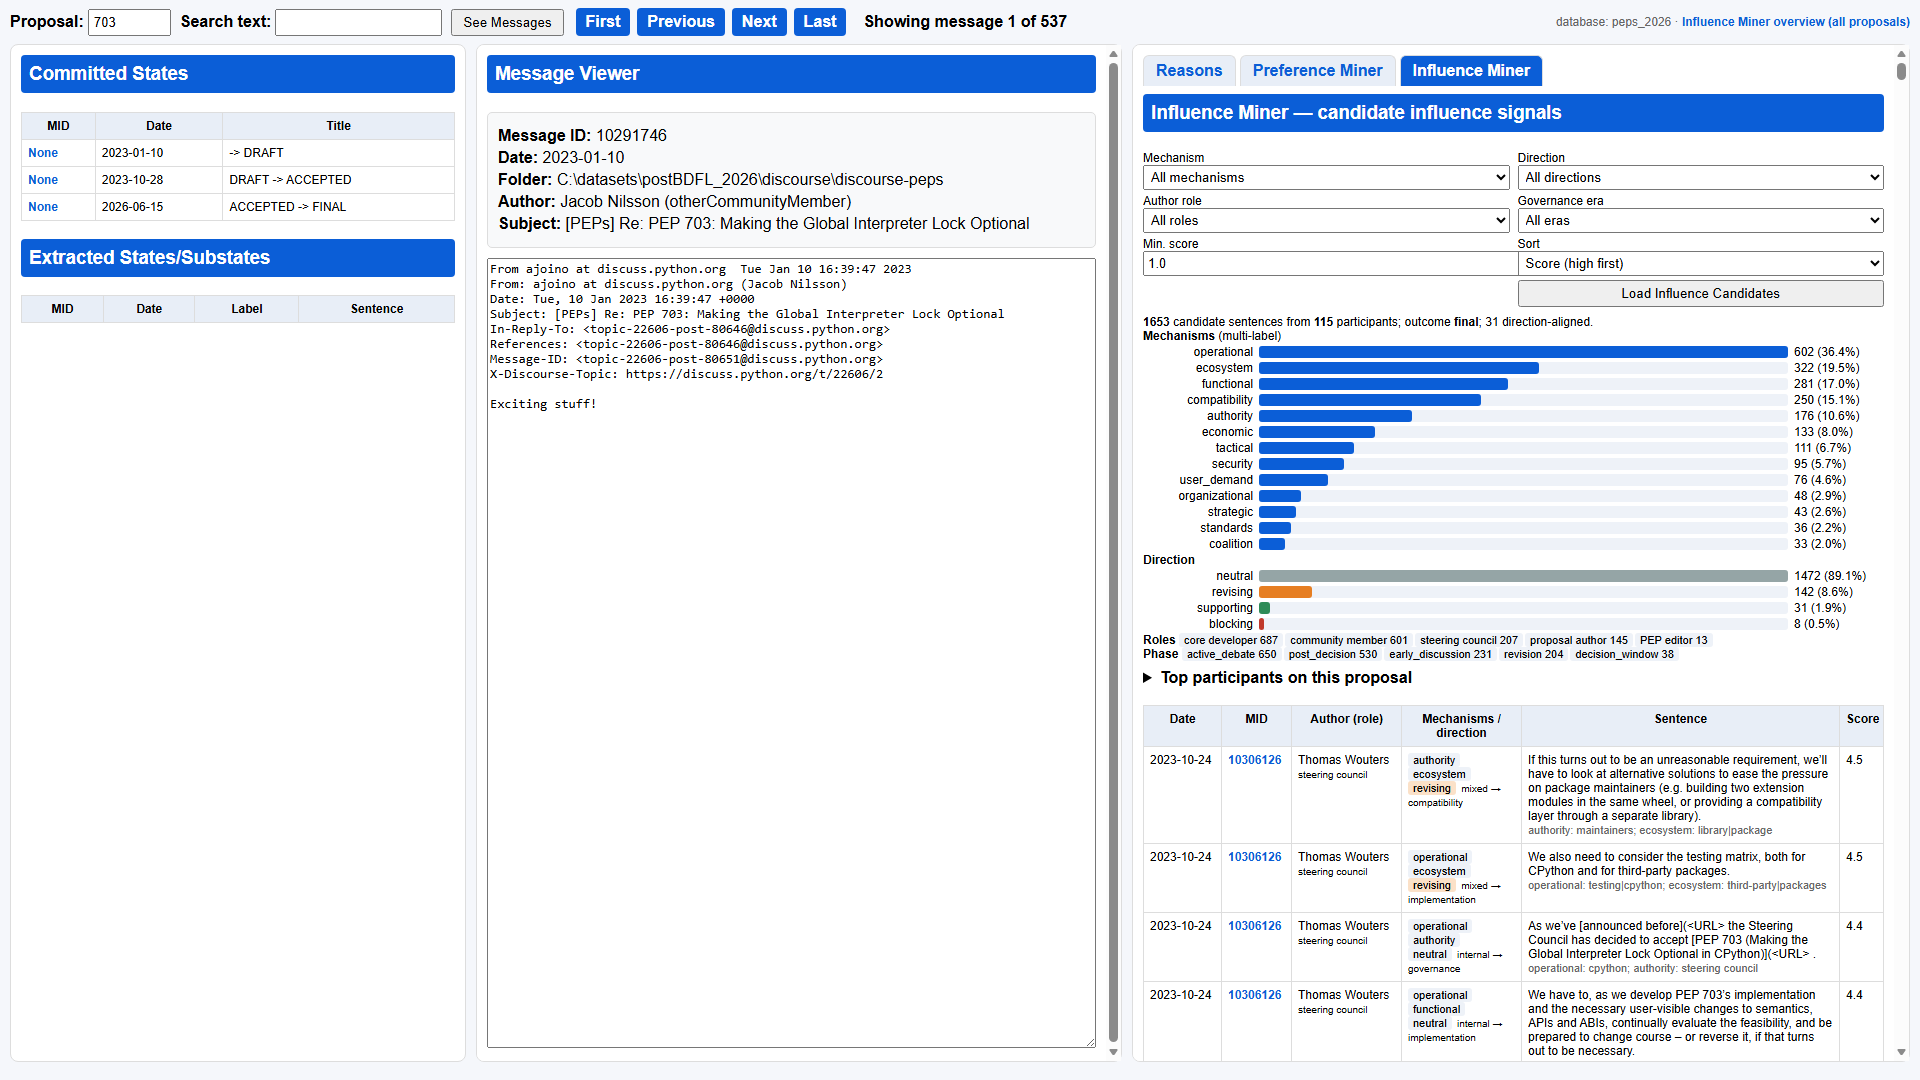
\includegraphics[width=\textwidth]{figures/fig_web_influence_tab_crop.png}
\caption{Influence Miner tab in the web version of DeMaP Miner (PEP~703, a Steering-Council-era proposal discussed on discuss.python.org). Left: the PEP's status history from the \texttt{python/peps} repository; centre: the selected Discourse post; right: filters, mechanism and direction bars, roles, phases and the candidate table.}
\Description{Screenshot of a browser window with three columns: committed states on the left, a message viewer in the middle, and on the right the Influence Miner tab with horizontal bars for thirteen mechanisms and four directions, role and phase tags, and the start of a candidate table.}
\label{fig:web}
\end{figure*}
